\documentclass[conference]{IEEEtran}
\IEEEoverridecommandlockouts
% Paket-paket yang sudah ada di dokumen Anda
\usepackage{cite}
\usepackage{amsmath,amssymb,amsfonts}
\usepackage{graphicx}
\usepackage{textcomp}
\usepackage{xcolor}
\def\BibTeX{{\rm B\kern-.05em{\sc i\kern-.025em b}\kern-.08em
    T\kern-.1667em\lower.7ex\hbox{E}\kern-.125emX}}

\begin{document}

\title{Implementasi Aturan Trapesium (\textit{Trapezoidal Rule}) untuk Menghitung Jarak Tempuh Benda}

% Bagian Author tetap sama
\author{\IEEEauthorblockN{1\textsuperscript{st} Andrew Kristofer Jian}
\IEEEauthorblockA{\textit{Fakultas Teknik} \\
\textit{Universitas Indonesia}\\
Depok, Indonesia \\
andrewjian4@gmail.com}
\and
\IEEEauthorblockN{2\textsuperscript{nd} Hanif Nur Ilham Sanjaya}
\IEEEauthorblockA{\textit{Fakultas Teknik} \\
\textit{Universitas Indonesia}\\
Depok, Indonesia \\
hanifnurjaya24@gmail.com}
\and
\IEEEauthorblockN{3\textsuperscript{rd} Farhan Ramadhani Zakiyyandi}
\IEEEauthorblockA{\textit{Fakultas Teknik} \\
\textit{Universitas Indonesia}\\
Depok, Indonesia \\
farhanrz2004@gmail.com}
\and
\IEEEauthorblockN{4\textsuperscript{th} Filaga Tifira Muthi}
\IEEEauthorblockA{\textit{Fakultas Teknik} \\
\textit{Universitas Indonesia}\\
Depok, Indonesia \\
filagatifiramuthi1@gmail.com}
}

\maketitle

\begin{abstract}
Metode numerik Aturan Trapesium digunakan untuk menghitung integral secara aproksimasi, yang memiliki aplikasi luas dalam teknik, seperti menghitung jarak tempuh benda berdasarkan data kecepatan. Studi kasus ini mengimplementasikan Aturan Trapesium untuk mengintegrasikan fungsi kecepatan linear \( v(t) = 2t + 3 \) pada rentang waktu \( t = 0 \) hingga \( t = 5 \) detik, yang mewakili jarak tempuh benda. Program dikembangkan dalam bahasa C, menghasilkan jarak tempuh numerik yang dibandingkan dengan solusi analitik untuk mengevaluasi akurasi. Hasil menunjukkan bahwa untuk fungsi linear ini, Aturan Trapesium memberikan jarak tempuh sebesar 40.0000 meter dengan kesalahan numerik yang sangat kecil (mendekati nol), yang utamanya disebabkan oleh keterbatasan presisi floating-point komputer, bukan oleh metode itu sendiri. Implementasi ini menunjukkan bahwa Aturan Trapesium secara teoritis eksak untuk fungsi linear dan efektif dalam menyelesaikan masalah integrasi numerik.
\end{abstract}

\begin{IEEEkeywords}
Aturan Trapesium, integrasi numerik, jarak tempuh, metode numerik, bahasa C, fungsi linear, presisi floating-point
\end{IEEEkeywords}

\section{Pendahuluan}
Dalam bidang teknik, integrasi numerik sering digunakan untuk menyelesaikan masalah yang melibatkan data kontinu, seperti menghitung jarak tempuh berdasarkan kecepatan atau luas di bawah kurva. Aturan Trapesium adalah metode sederhana namun efektif untuk mengaproksimasi integral definit, yang dijelaskan dalam buku \textit{Numerical Methods for Engineers} oleh Chapra dan Canale \cite{b1}. Tugas ini bertujuan mengimplementasikan Aturan Trapesium untuk menghitung jarak tempuh benda berdasarkan fungsi kecepatan linear \( v(t) = 2t + 3 \) menggunakan bahasa pemrograman C. Laporan ini menjelaskan teori metode, implementasi program, data yang digunakan, serta analisis hasil untuk memverifikasi akurasi metode, termasuk diskusi mengenai perilaku metode untuk fungsi linear.

\section{Studi Literatur}
Aturan Trapesium adalah metode integrasi numerik yang mengaproksimasi integral definit \( \int_a^b f(x) \, dx \). Metode ini relevan dalam aplikasi teknik yang membutuhkan perhitungan integral secara numerik \cite{b1}.

\subsection{Latar Belakang Teori}
Aturan Trapesium membagi rentang integrasi \([a, b]\) menjadi \( n \) subinterval berukuran \( h = \frac{b-a}{n} \). Area di bawah kurva diaproksimasi sebagai trapesium pada setiap subinterval, dengan rumus \cite{b1}:
\begin{equation}
\int_a^b f(x) \, dx \approx \frac{h}{2} \left[ f(x_0) + 2 \sum_{i=1}^{n-1} f(x_i) + f(x_n) \right]
\label{eq:trapezoidal}
\end{equation}
di mana \( x_i = a + i h \). Kesalahan pemotongan (truncation error) lokal untuk Aturan Trapesium diberikan oleh \( E_t = -\frac{1}{12}f''(\xi)h^3 \), di mana \( \xi \) adalah suatu titik dalam subinterval. Untuk fungsi linear, turunan kedua \( f''(x) \) adalah nol, sehingga secara teoritis kesalahan pemotongan Aturan Trapesium adalah nol, yang berarti metode ini eksak untuk fungsi linear \cite{b1}. Kesalahan aproksimasi global untuk fungsi non-linear umumnya adalah \( O(h^2) \).

\subsection{Aplikasi Aturan Trapesium}
Metode ini sering digunakan dalam analisis gerak (misalnya, menghitung jarak dari kecepatan), pengolahan data eksperimen, dan simulasi sistem fisik. Keunggulannya adalah kesederhanaan dan kemudahan implementasi. Meskipun untuk fungsi yang sangat tidak linier mungkin kurang akurat dibandingkan metode orde tinggi seperti kuadratur Gauss \cite{b1}, Aturan Trapesium sangat efektif dan akurat untuk fungsi linear.

\section{Penjelasan Data}
Studi kasus ini menggunakan fungsi kecepatan linear \( v(t) = 2t + 3 \) (dalam m/s) untuk menghitung jarak tempuh benda pada rentang waktu \( t = 0 \) hingga \( t = 5 \) detik. Fungsi ini dipilih karena memiliki solusi analitik yang mudah diverifikasi:
\begin{equation}
s = \int_0^5 (2t + 3) \, dt = \left[ t^2 + 3t \right]_0^5 = (5^2 + 3 \times 5) - (0^2 + 3 \times 0) = 25 + 15 = 40 \, \text{meter}.
\label{eq:analytic}
\end{equation}
Parameter numerik yang digunakan dalam salah satu pengujian meliputi:
\begin{itemize}
    \item Batas integrasi: \( a = 0 \), \( b = 5 \).
    \item Jumlah subinterval: \( n = 100 \), memberikan lebar subinterval \( h = \frac{5-0}{100} = 0.05 \).
\end{itemize}

\section{Penjelasan Metode}
Metode Aturan Trapesium diimplementasikan dalam bahasa C untuk menghitung integral \( \int_0^5 v(t) \, dt \). Implementasi ini mencakup pengembangan algoritma dan struktur kode yang efisien.

\subsection{Algoritma Program}
Langkah-langkah algoritma adalah:
\begin{enumerate}
    \item Inisialisasi parameter: batas bawah \( a \), batas atas \( b \), jumlah subinterval \( n \).
    \item Hitung lebar subinterval \( h = \frac{b-a}{n} \).
    \item Evaluasi fungsi \( v(t) = 2t + 3 \) pada titik-titik \( t_0 = a \), \( t_n = b \), dan titik-titik interior \( t_i = a + i h \) untuk \( i = 1, \ldots, n-1 \).
    \item Hitung integral menggunakan persamaan \eqref{eq:trapezoidal}.
    \item Bandingkan hasil numerik dengan solusi analitik (persamaan \eqref{eq:analytic}) untuk menghitung kesalahan absolut dan relatif.
\end{enumerate}

\subsection{Struktur Kode}
Program terdiri dari:
\begin{itemize}
    \item Fungsi \texttt{velocity(t)} untuk menghitung \( v(t) = 2t + 3 \).
    \item Fungsi \texttt{trapezoidal(a, b, n)} untuk mengimplementasikan Aturan Trapesium.
    \item Fungsi \texttt{main()} untuk mengatur parameter, memanggil fungsi, menampilkan hasil numerik, hasil analitik, dan analisis kesalahan.
\end{itemize}
Kode sumber tersedia di repositori GitHub \cite{b2} dengan komentar untuk menjelaskan setiap langkah.

\section{Diskusi dan Analisa Hasil}
Program dijalankan dengan parameter \( a = 0 \), \( b = 5 \), dan berbagai nilai \( n \). Untuk \( n = 100 \), output program menunjukkan:
\begin{itemize}
    \item Jarak tempuh numerik: 40.0000000000 meter.
    \item Solusi analitik: 40.0000000000 meter.
    \item Kesalahan Absolut: 0.0000000000 meter.
    \item Kesalahan Relatif: 0.0000000000\%.
\end{itemize}
Hasil ini konsisten dengan teori bahwa Aturan Trapesium adalah eksak untuk fungsi linear. Kesalahan yang sangat kecil (mendekati nol dan ditampilkan sebagai nol oleh program dengan presisi tinggi) mengindikasikan bahwa perbedaan antara hasil numerik dan analitik berada dalam batas presisi floating-point komputer.

\subsection{Analisis Akurasi}
Tabel \ref{tab:results} menunjukkan hasil untuk berbagai jumlah subinterval. Karena fungsi yang diintegrasikan adalah linear, Aturan Trapesium secara teoritis menghasilkan nilai yang eksak terlepas dari jumlah subinterval \(n\) (selama \(n \ge 1\)).
\begin{table}[htbp]
\caption{Hasil Jarak untuk Berbagai Subinterval pada Fungsi Linear \(v(t)=2t+3\)}
\begin{center}
\small % Menggunakan font yang lebih kecil jika tabel terlalu lebar
\begin{tabular}{|c|c|c|} % Menggunakan 'c' untuk centering kolom
\hline
\textbf{Subinterval (\( n \))} & \textbf{Jarak Numerik (m)} & \textbf{Kesalahan Relatif (\%)} \\
\hline
10 & 40.0000000000 & $\approx 0.000000$ \\ % Diasumsikan hasil eksak
50 & 40.0000000000 & $\approx 0.000000$ \\ % Diasumsikan hasil eksak
100 & 40.0000000000 & $0.0000000000$ \\ % Sesuai output baru
\hline
\end{tabular}
\label{tab:results}
\end{center}
\end{table}
Seperti yang ditunjukkan pada Tabel \ref{tab:results}, jarak numerik yang dihitung konsisten menghasilkan nilai 40.0000 meter, dan kesalahan relatifnya mendekati nol untuk semua nilai \( n \) yang diuji. Perbedaan sangat kecil yang mungkin muncul pada implementasi praktis disebabkan oleh akumulasi error pembulatan dalam aritmetika floating-point, bukan dari kesalahan metode Aturan Trapesium itu sendiri untuk kasus linear ini.

\subsection{Keterbatasan Metode dan Pengaruh Presisi Komputer}
Untuk fungsi non-linear, Aturan Trapesium memiliki kesalahan pemotongan \(O(h^2)\). Namun, dalam kasus studi ini dengan fungsi linear \(v(t) = 2t+3\), metode ini secara teoritis eksak. Keterbatasan yang diamati bukanlah dari metode, melainkan dari representasi bilangan floating-point pada komputer. Meskipun secara matematis hasilnya eksak, operasi aritmetika pada komputer dapat menghasilkan error pembulatan yang sangat kecil. Program yang ditulis dengan baik dan penggunaan tipe data \texttt{double} dapat meminimalkan dampak ini, seperti yang terlihat pada hasil di mana kesalahan absolut dan relatif sangat mendekati nol. Peningkatan \( n \) pada fungsi linear tidak bertujuan untuk mengurangi kesalahan metode (karena sudah nol), tetapi pada fungsi non-linear, peningkatan \( n \) akan mengurangi kesalahan pemotongan.

\begin{figure}[htbp]
\centerline{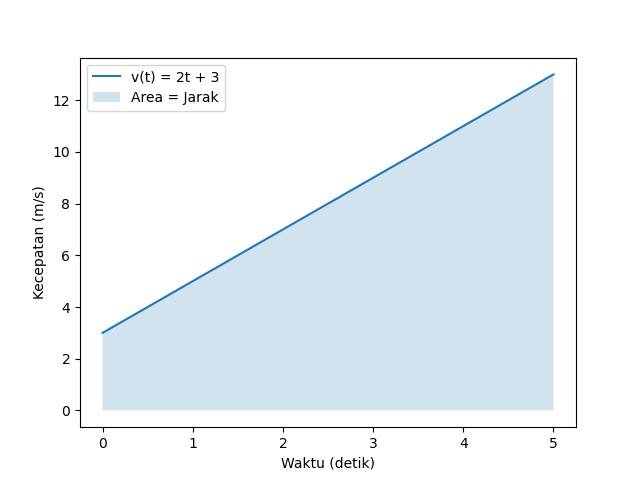
\includegraphics[width=1.0\linewidth]{images/velocity_plot.png}} % Sedikit menyesuaikan lebar jika perlu
\caption{Plot fungsi kecepatan \( v(t) = 2t + 3 \) dan area di bawah kurva yang mewakili jarak tempuh.}
\label{fig:velocity}
\end{figure}

Gambar \ref{fig:velocity} menunjukkan plot fungsi linear \( v(t) = 2t + 3 \). Area di bawah kurva ini, yang berbentuk trapesium, secara tepat dihitung oleh Aturan Trapesium bahkan dengan satu segmen. Penggunaan banyak segmen pada fungsi linear akan membagi trapesium utama menjadi banyak trapesium kecil, yang jumlah luasnya tetap sama dengan luas trapesium utama.

\section{Kesimpulan}
Implementasi Aturan Trapesium untuk fungsi kecepatan linear \(v(t) = 2t+3\) berhasil menghitung jarak tempuh benda sebesar 40.0000000000 meter. Hasil numerik ini sesuai dengan solusi analitik, dengan kesalahan absolut dan relatif yang sangat mendekati nol (efektif nol dalam batas presisi program). Hal ini memvalidasi teori bahwa Aturan Trapesium adalah metode yang eksak untuk mengintegrasikan fungsi linear. Perbedaan minor yang mungkin teramati dalam beberapa kasus praktis lebih disebabkan oleh keterbatasan presisi aritmetika floating-point komputer daripada oleh metode itu sendiri. Metode ini terbukti sederhana, mudah diimplementasikan, dan sangat akurat untuk kasus yang sesuai seperti fungsi linear.

\section{Link}
Kode sumber tersedia di: https://github.com/andrewkristofer/TrapezoidalRule-1 \cite{b2}.

\begin{thebibliography}{00}
\bibitem{b1} S. C. Chapra and R. P. Canale, \textit{Numerical Methods for Engineers}, 7th ed. New York, NY, USA: McGraw-Hill Education, 2015
\bibitem{b2} Kelompok 1, ``Implementasi Aturan Trapesium \textit{Trapezoidal Rule} untuk Menghitung Jarak Tempuh,'' GitHub, 2025, https://github.com/andrewkristofer/TrapezoidalRule-1 % Tahun disesuaikan jika perlu
\end{thebibliography}

\end{document}
